\chapter{Implementasi dan Pengujian}
\label{chap:implementasi&pengujian}

Pada bab ini akan dijelaskan mengenai implementasi perangkat lunak, serta pengujian perangkat lunak. Implementasi perangkat lunak berisi penjelasan lingkungan pengembangan perangkat lunak dan hasil implementasi. Sedangkan pengujian perangkat lunak berisi hasil pengujian fungsional dan eksperimental terhadap perangkat lunak yang telah dibangun.

\section{Implementasi}

\subsection{Lingkungan Implementasi}
\label{lingkungan_implementasi}
Implementasi perangkat lunak ini dilakukan di komputer penulis dengan spesifikasi berikut:
\begin{enumerate}
    \item \textit{Processor}: Intel Core i5-10300H
    \item \textit{Random Access Memory(RAM)}: 16 GB DDR4
    \item Sistem Operasi: Windows 10
    \item Versi Java: 1.8.0\_291
    \item Versi JavaFX: 8.0.202
    \item Versi Netbeans: 12.1
    \item Versi Scenebuilder: 11.0.0
\end{enumerate}

\subsection{Hasil Implementasi}
Implementasi berupa aplikasi \textit{screensaver}, dimana aplikasi tersebut akan dijalankan secara otomatis setelah komputer tidak digunakan selama beberapa saat. Gambar \ref{fig:5_hasil} dan \ref{fig:5_hasil2} merupakan tampilan dari aplikasi \textit{screensaver}. Dikarenakan pada Portal Akademik Mahasiswa tidak terdapat foto mahasiswa, maka foto digantikan dengan \textit{base64 image} yang dimasukkan secara \textit{hardcode}. \textit{Layout} dari aplikasi disimpan dalam \textit{file} bertipe FXML (lampiran ...). \textit{file} FXML tersebut tidak dibuat secara manual, melainkan dengan menggunakan aplikasi Scene Builder\footnote{\url{https://gluonhq.com/products/scene-builder/}}. 

\begin{figure}[H]
	\centering
	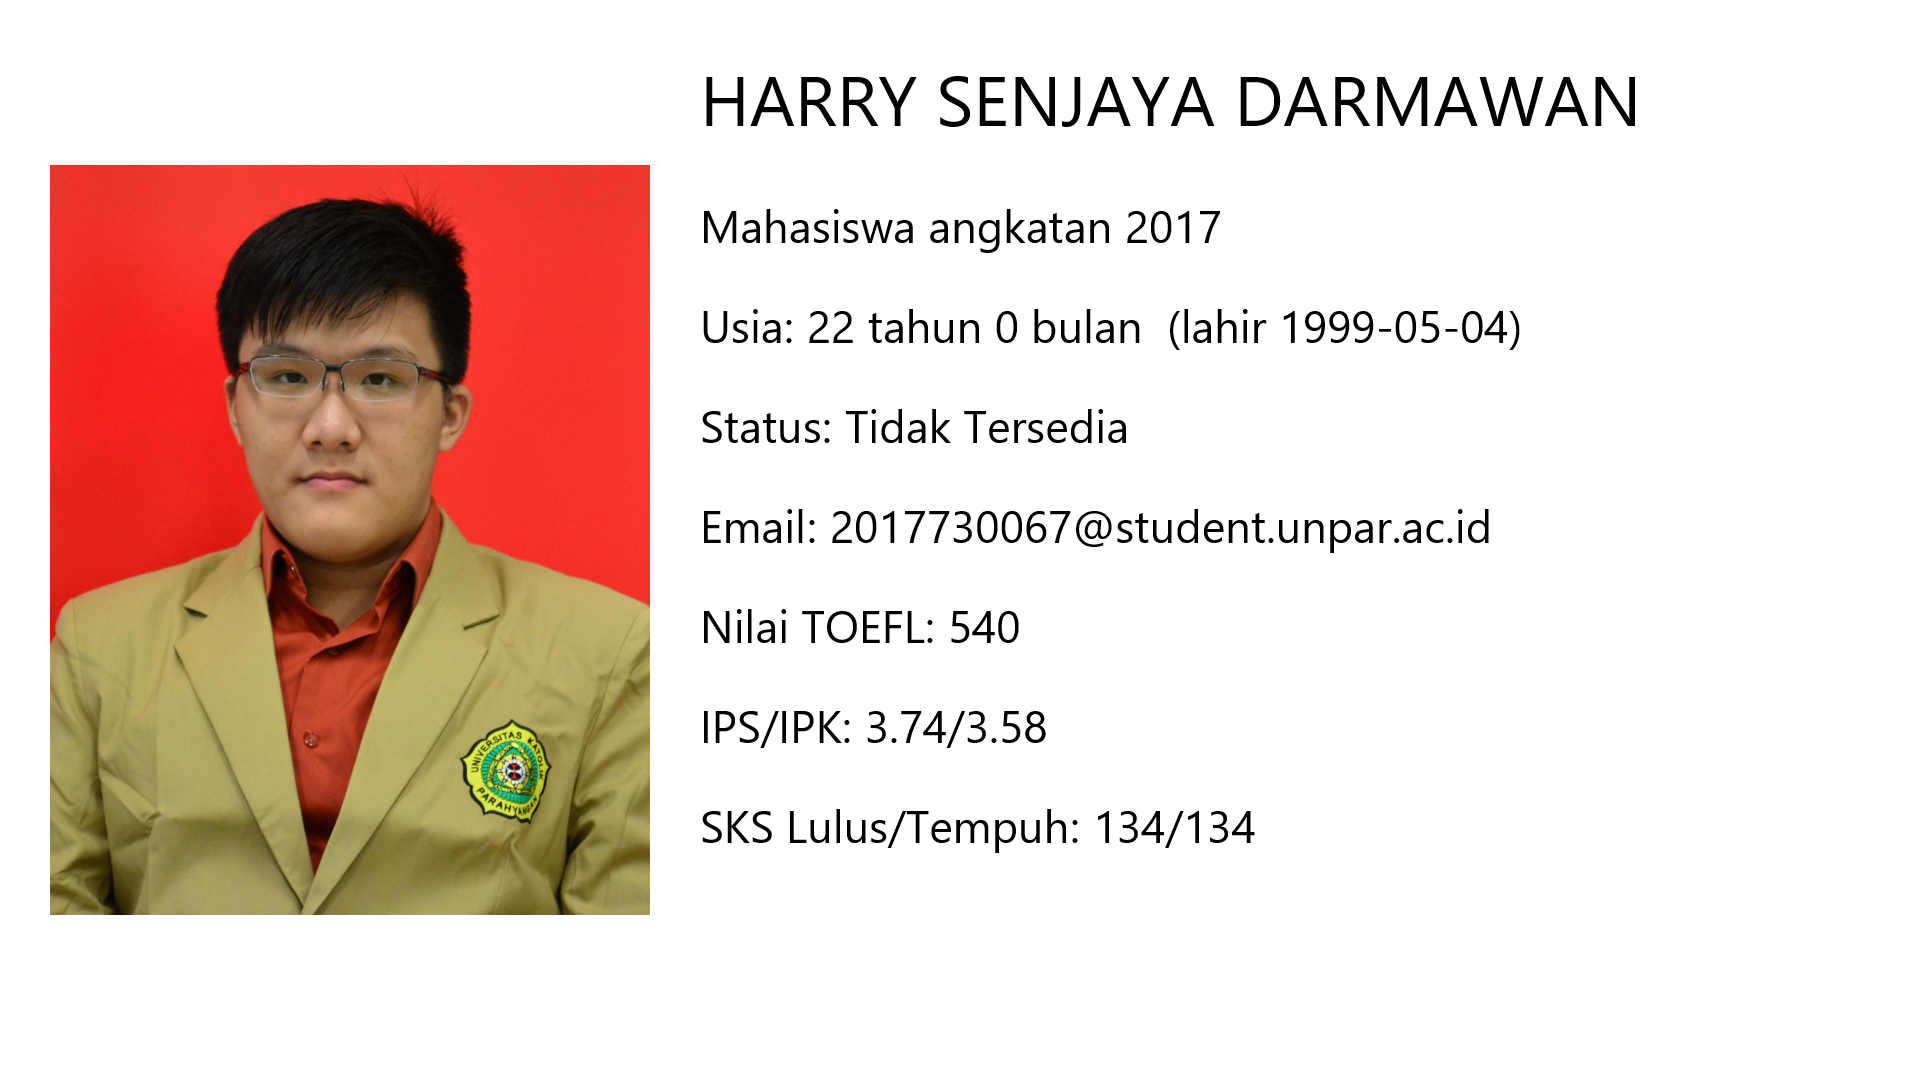
\includegraphics[scale=0.3]{Gambar/hasil.png}
	\caption{Tampilan \textit{Screensaver} Mahasiswa Pertama}
	\label{fig:5_hasil}
\end{figure}

\begin{figure}[H]
	\centering
	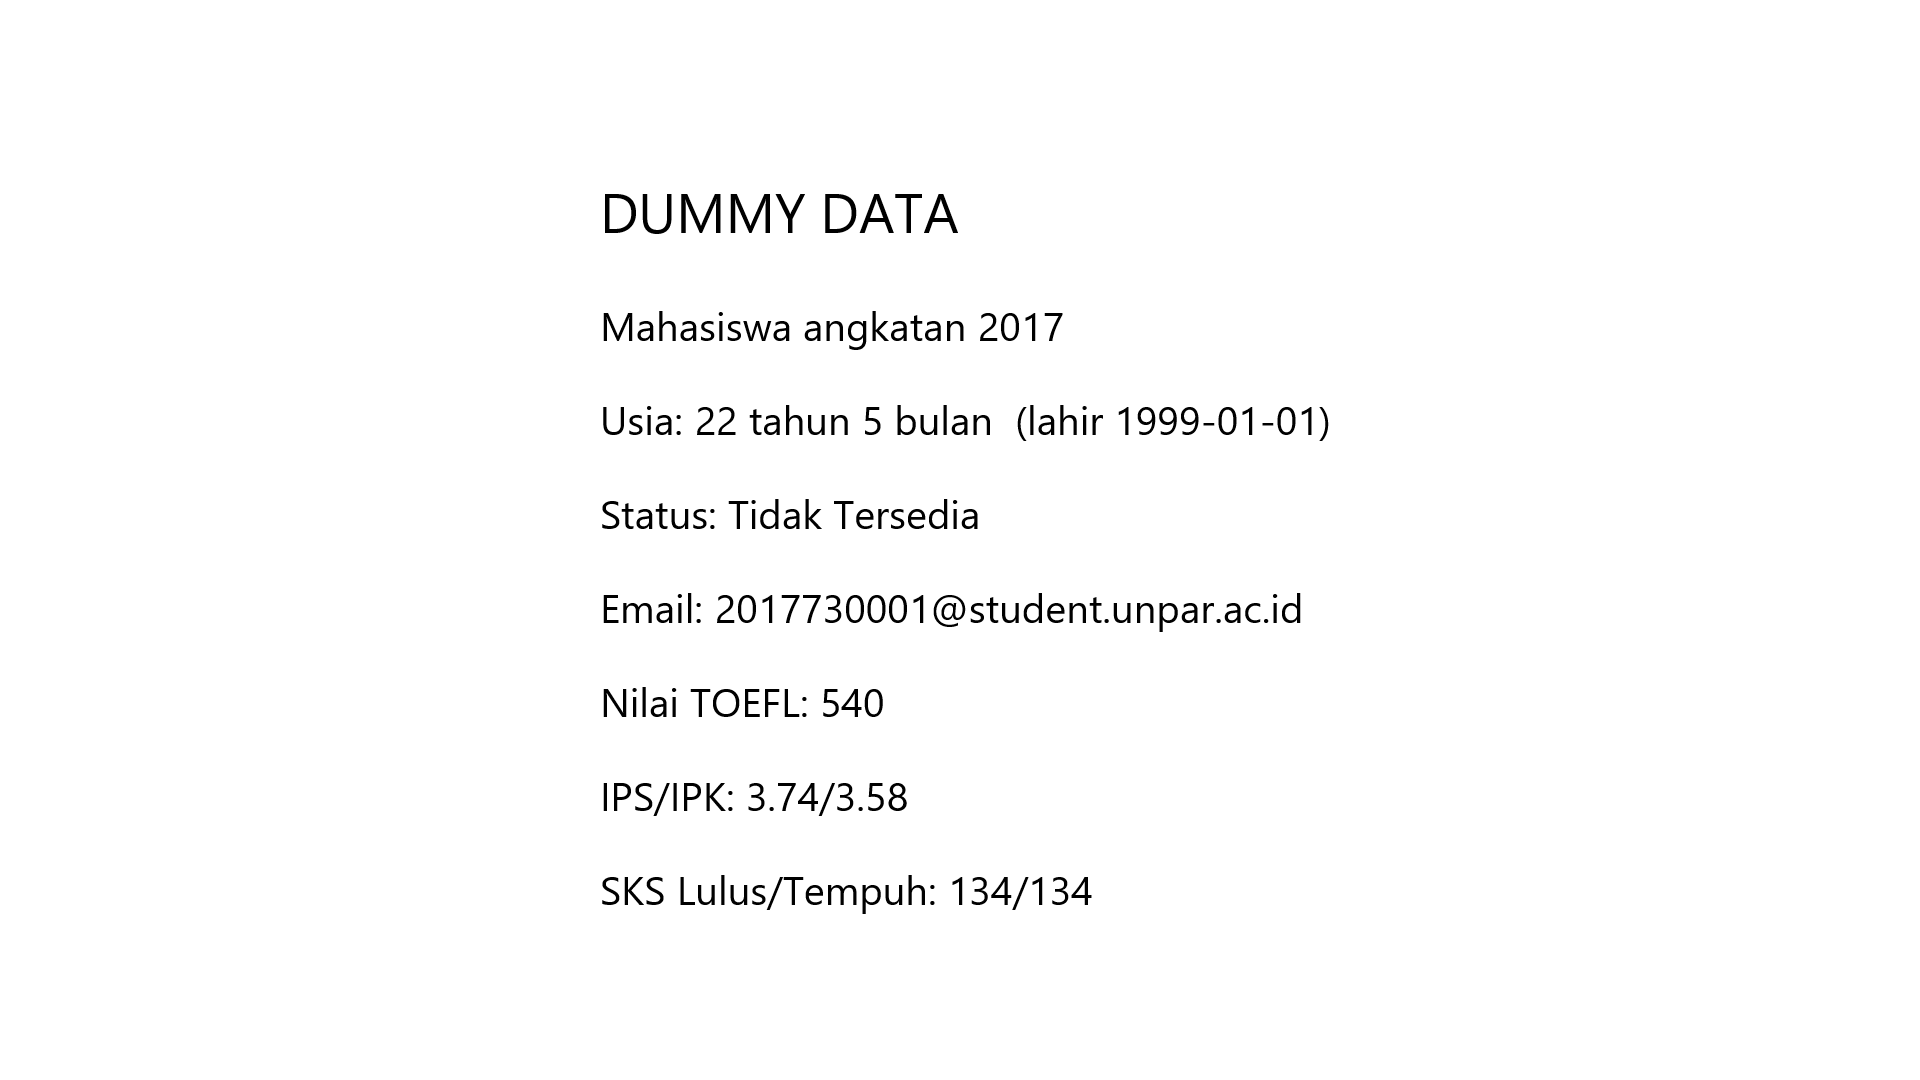
\includegraphics[scale=0.3]{Gambar/hasil2.png}
	\caption{Tampilan \textit{Screensaver} Mahasiswa Kedua}
	\label{fig:5_hasil2}
\end{figure}


\section{Pengujian}

\section{Pengujian Fungsional}
Pengujian fungsional dilakukan untuk mengetahui kesesuaian reaksi perangkat lunak dengan reaksi yang diharapkan berdasarkan aksi pengguna terhadap perangkat lunak. Tabel \ref{table:hasilFungsional} merupakan hasil pengujian perangkat lunak yang dilakukan di komputer penulis dengan spesifikasi berikut:
\begin{enumerate}
    \item \textit{Processor}: Intel Core i5-10300H
    \item \textit{Random Access Memory(RAM)}: 16 GB DDR4
    \item Sistem Operasi: Windows 10
    \item Resolusi Layar: 1920 x 1080
    \item Versi Java: 1.8.0\_291
\end{enumerate}

\begin{table}[H]
	\centering
	\caption{Tabel Pengujian Fungsional}
	\begin{tabular}{|p{0.5cm}| p{5.5cm}| p{5.5cm}| p{3cm}|} \hline
	No.	&	Aksi Pengguna	&	Reaksi yang diharapkan	&	Reaksi Perangkat Lunak \\ \hline
	1.	&	Dosen atau mahasiswa tidak menggunakan komputer selama beberapa saat. 	&	\textit{Screensaver} berjalan dengan menampilkan biodata dan data akademik mahasiswa secara umum.	&	sesuai	\\ \hline
	\end{tabular}
	\label{table:hasilFungsional}
\end{table}


\section{Pengujian Eksperimental}
\textit{Subbab ini ditulis oleh dosen pembimbing.}
